% \documentclass[8pt,xcolor=pdftex,table,handout]{beamer}

\documentclass[8pt,xcolor=pdftex,table]{beamer}
\include{preambule_beamer}

\usepackage{listings}

% \usepackage{amsmath}
% \usepackage{unicode-math}
% \setmathfont{Fira Math}


% \usepackage{animate}

% ------------------------------------------- %

\graphicspath{{Figures/} {Figures/Logos/} {../Figures/}}
% \graphicspath{{../Figures/} {../Figures/Logos/}}

\title[]{\vspace{22mm}Formation \alert{Ingénieur Machine Learning}\\\vspace{6mm}Projet:\\Segmentez des clients d'un site e-commerce}
\date[]{\alert{XX} Avril 2023\\\vspace{18mm}\\\tit{thomas.durandtexte@protonmail.com}}


\titlegraphic{\hfill
\def\arraystretch{.1}%  1 is the default, change whatever you need
	\begin{tabular}{ >{\centering}m{7mm} m{39mm} }
		
\includegraphics[height=7mm]{Logo_OpenClassrooms.png }
		&
		\Large{\textbf{OPENCLASSROOMS}}
	\end{tabular}
}

\definecolor{blueOlist}{rgb}{0.063,0.157,0.816}

\definecolor{clrE1}{rgb}{1,0.7,0}
\definecolor{clrE2}{rgb}{1,0.6,0}
\definecolor{clrE3}{rgb}{1,0.5,0}
\definecolor{clrE4}{rgb}{1,0.4,0}
\definecolor{clrE5}{rgb}{1,0.3,0}

\definecolor{clrData}{rgb}{0.9,0.5,0}

\tikzstyle{box_style00}=[draw, rounded corners,anchor=center,text centered,text=white]
\tikzstyle{diagram0}=[box_style00, text width=22mm, minimum height=12mm]
\tikzstyle{dataset}=[box_style00,diagram0, fill=blue]
\tikzstyle{filtrage}=[box_style00,diagram0, fill=red!80]
\tikzstyle{doublons}=[box_style00,diagram0, fill=magenta!80]
\tikzstyle{datavoisins}=[box_style00,diagram0, fill=cyan!80]
\tikzstyle{outliers}=[box_style00,diagram0, fill=magenta!80]

% \includeonlyframes{Merci}



\begin{document}
% ------------------------------------------- %

\begin{frame}
	\titlepage{}
\end{frame}


\section{CONTEXTE}


\begin{frame}[t, label=contexte]
	\vspace{0mm}
	\begin{tikzpicture}
		\linespread{1}% <--- locally defined vertical line spacing in nodes
		\draw[clrBorders] (0,0) rectangle (\txw,\txh) ;
		\nodePageNumber

		\node[fill=blueOlist, text centered, minimum width=10mm, minimum height=10mm]
			(A) at (20mm,80mm) { olist } ;

		\visible<2->{
			\node[box_style00, text width = 40mm] (B) at (\midX+20mm,80mm) { Solution de \alert{vente} sur les \alert{marketplaces en ligne}\\(Brésil) } ;
			\draw[myarrow, <->] (A) -- (B) ;
		}
		\visible<3->{
			\node[box_style00, text width=70mm] (C)
				at (\midX,60mm) { Demande d'une \alert{segmentation clients} avec \alert{description actionnable} } ;
			\draw[myarrow] (B) -- ++(0, -9mm) -| (C) ;
		}

		\visible<4->{
			\node[box_style00, text width=70mm] (D) at (\midX,40mm) { Objectif :\\\alert{aide} pour les campagnes de \alert{communication}\\de l'équipe marketing} ;
			\draw[myarrow] (C) -- (D) ;
		}

		\visible<5>{
			\node[box_style00, text width=70mm] at (\midX,20mm) { À prévoir :\\proposition de \alert{contrat de maintenance} } ;
		}

	\end{tikzpicture}
\end{frame}

\subsection{Base de données}
\begin{frame}[t, label=BaseDonnees]
	\vspace{0mm}
	\begin{tikzpicture}
		\linespread{1}% <--- locally defined vertical line spacing in nodes
		\draw[clrBorders] (0,0) rectangle (\txw,\txh) ;
		\nodePageNumber

		\node[myShaded] at (\midX, 80mm) {Base de données fournie} ;
		\node[draw, rounded corners, fill=black!4] at (\midX, \midY) { 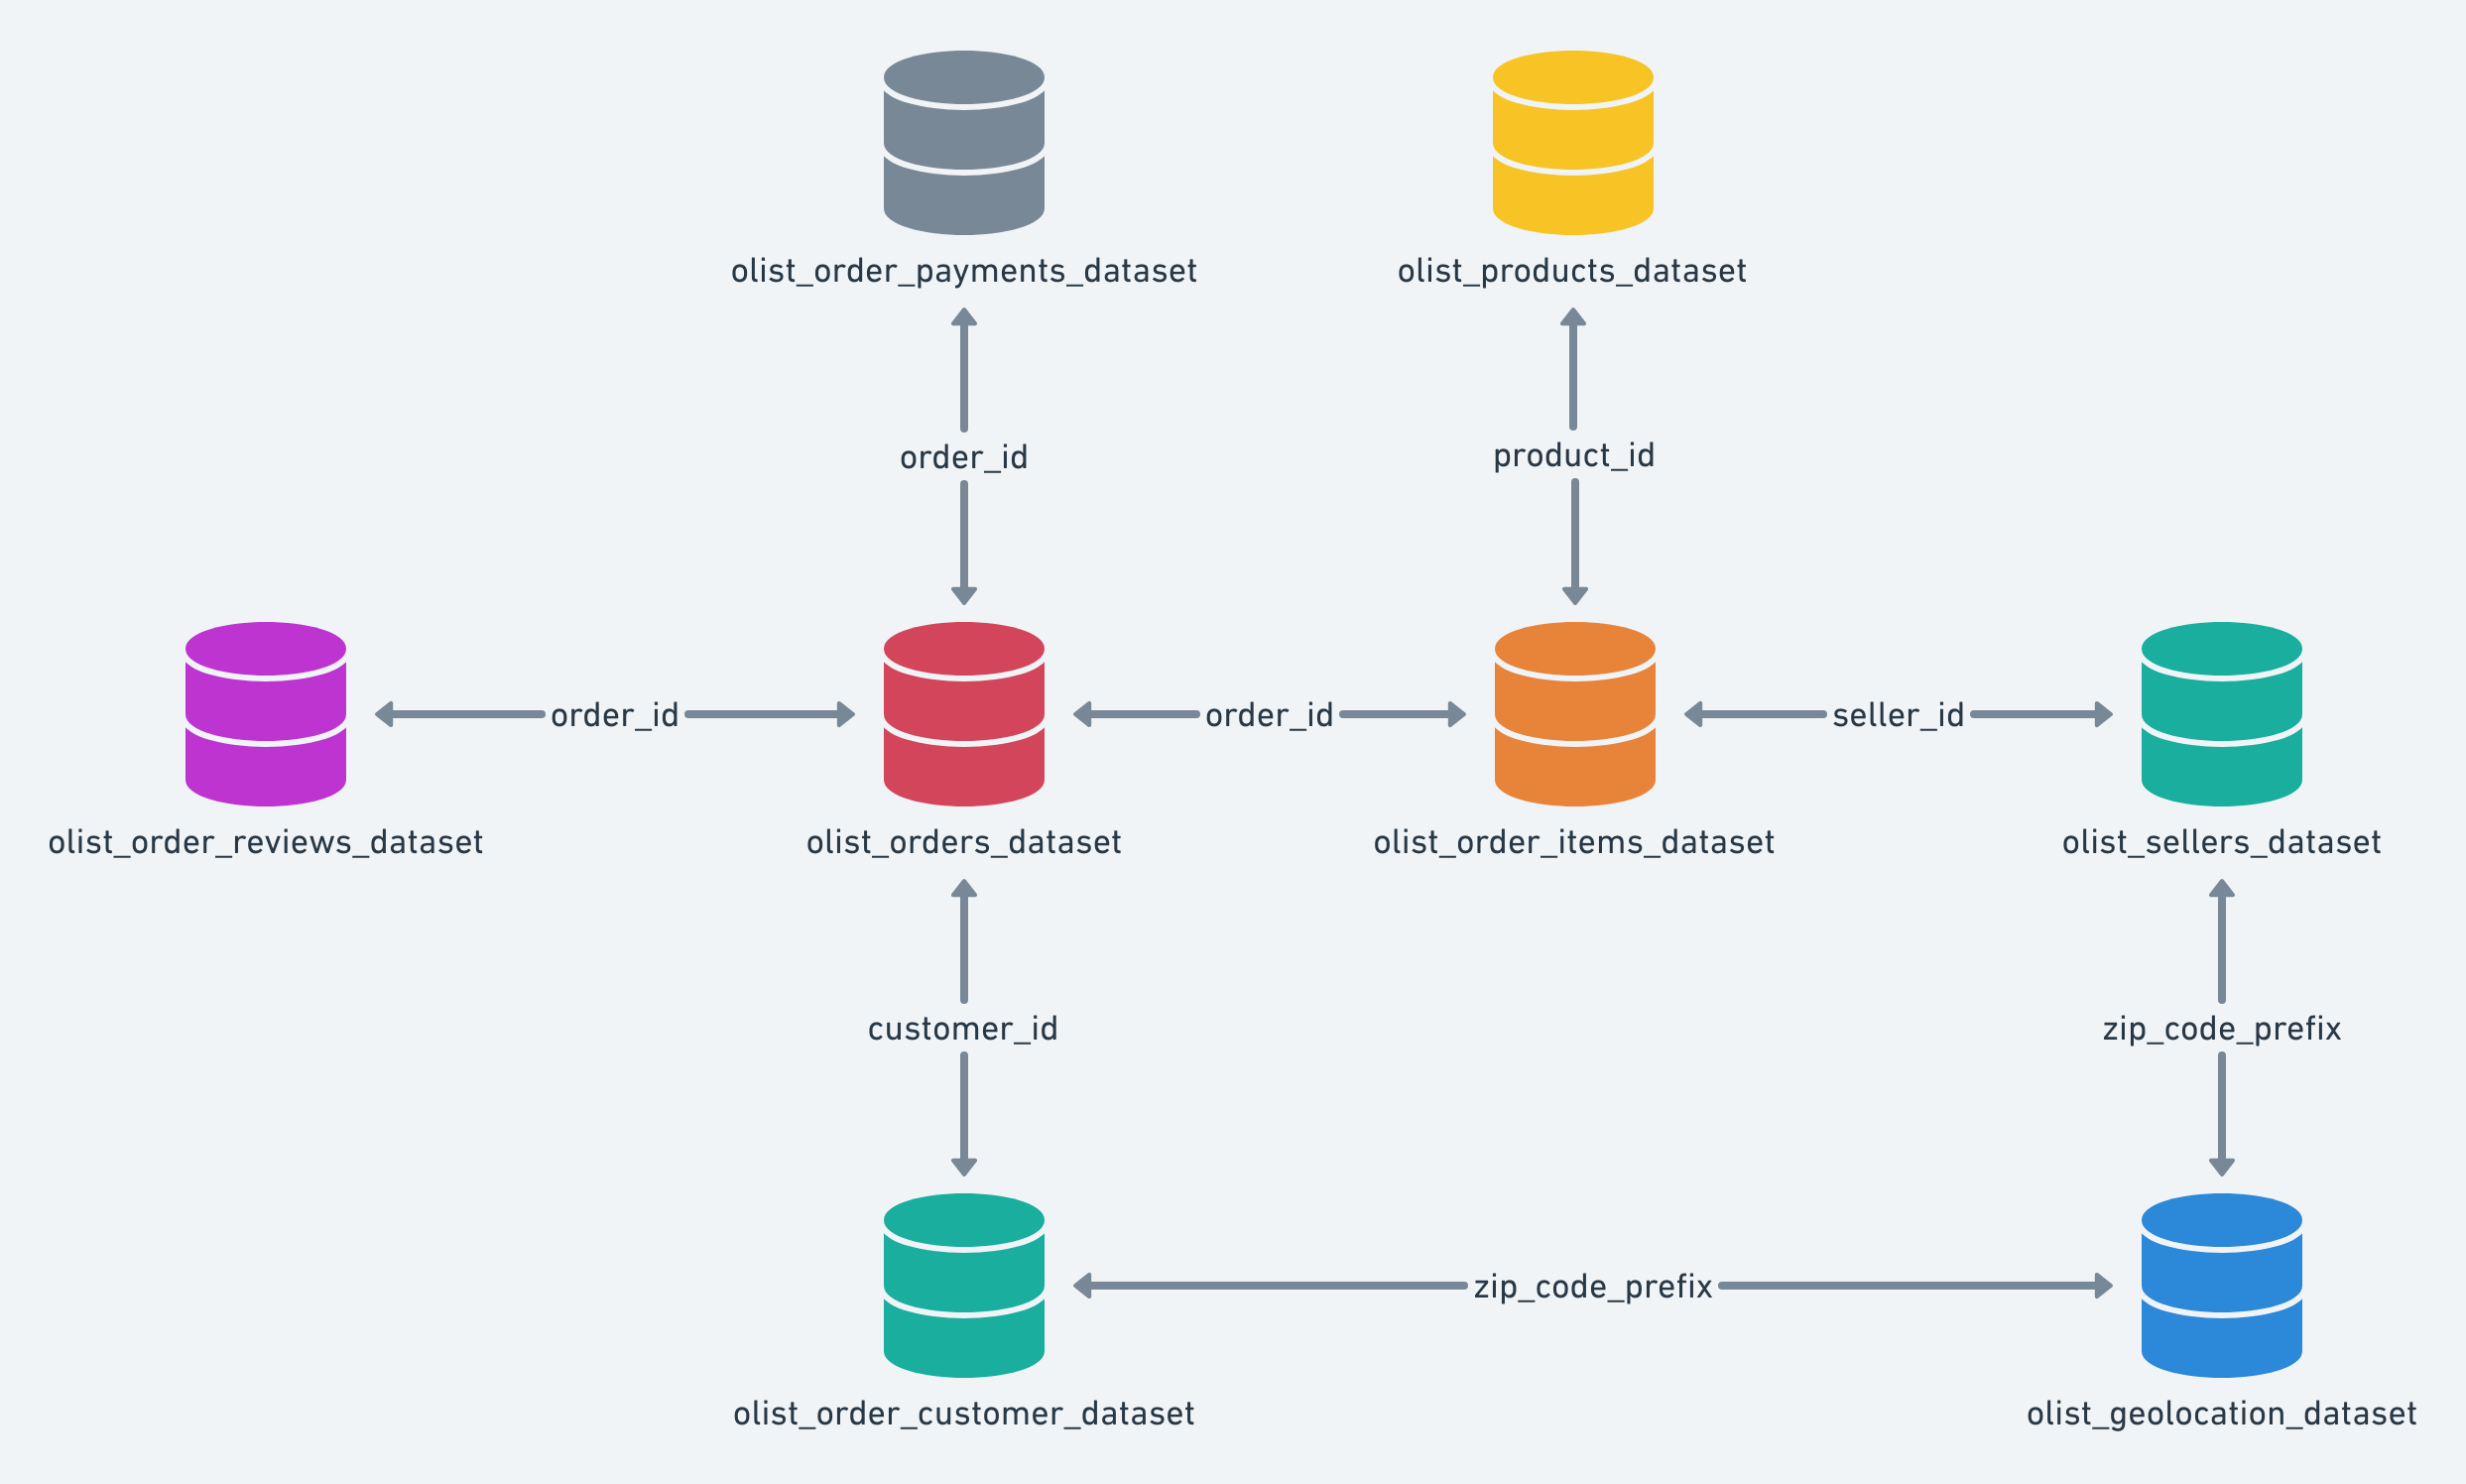
\includegraphics[width=90mm]{data_diagram.png}} ;

		\visible<2->{
			\node[myOrng, text centered, text width=10mm] at (21mm,65mm) {Données étudiées} ;
		}

		\node (A) at (35mm, 40.25mm) {} ;
		\visible<2>{
			\draw[myOrng, thick, rounded corners] (A.center) -- ++( 0, 11.5mm) --++ ( 18.2mm, 0) -- ++(0,-11.5mm) -- cycle ;
		}

		\visible<3>{
			\draw[myOrng, thick, rounded corners] (A.center) -- ++( 0, 32.3mm) --++ ( 18.2mm, 0) -- ++(0,-32.3mm) -- cycle ;
		}

		\visible<4>{
			\draw[myOrng, thick, rounded corners] (A.center) -- ++( 0, 32.3mm) --++ ( 18.2mm, 0) -- ++(0,-53mm) -- ++(-18.2mm,0) -- cycle ;
		}


		\visible<5>{
			\draw[myOrng, thick, rounded corners] (A.center) -- ++(-25.2mm, 0) -- ++(0, 11.5mm) --++(25.2mm,0) --++( 0, 32.3mm-11.5mm) --++ ( 18.2mm, 0) -- ++(0,-53mm) -- ++(-18.2mm,0) -- cycle ;
		}

	\end{tikzpicture}
\end{frame}


\subsection{Protocole}
\begin{frame}[t, label=protocol]
	\vspace{0mm}
	\begin{tikzpicture}
		\linespread{1}% <--- locally defined vertical line spacing in nodes
		\draw[clrBorders] (0,0) rectangle (\txw,\txh) ;
		\nodePageNumber

		\node[box_style00, text width=25mm] (A) at (25mm,80mm) {Construction des \alert{variables RFM}} ;

		\visible<2->{
			\node[box_style00, text width=25mm] (B) at (80mm,80mm) {Essais avec \alert{différents modèles}} ;
			\draw[myarrow] (A) -- (B) ;
		}

		\visible<3->{
			\node[box_style00, below=of B] (C) {\alert{Sélection} d'un modèle} ;
			\draw[myarrow] (B) -- (C) ;
		}

		\visible<4->{
			\node[box_style00] (D) at (25mm,50mm) {\alert{Ajout} de \alert{variables}} ;
			\draw[myarrow] (A) -- (D) ;
		}

		\visible<5->{
			\node[box_style00] (E) at (80mm,50mm) {\alert{Analyse} de la \alert{pertinence}} ;
			\draw[myarrow] (D) -- (E) ;
			\draw[myarrow] (C) -- (E) ;
		}

		\visible<6>{
		\node[box_style00, text width=60mm] (F) at (\midX,20mm) {\alert{Estimation} de la \alert{fréquence} requise pour la \alert{maintenance} de la segmentation} ;
		\draw[myarrow, line width=2pt] (\midX, 35mm) -- (F) ;
		\draw[decorate, line width=2pt, decoration={brace, mirror, amplitude=7mm}]
			(0.07*\txw, 42mm) -- ++ (0.86*\txw, 0) ;
		}

	\end{tikzpicture}
\end{frame}


\section{EXPLORATION DES DONNÉES}

\subsection{Évolution temporelle du nombre de commandes}

\begin{frame}[t, label=n_orders_vs_tim]
	\vspace{0mm}
	\begin{tikzpicture}
		\linespread{1}% <--- locally defined vertical line spacing in nodes
		\draw[clrBorders] (0,0) rectangle (\txw,\txh) ;
		\nodePageNumber

		\node[myShaded] at (\midX,80mm) {Évolution temporelle du nombre de commandes} ;
		\node at (\midX,\midY) {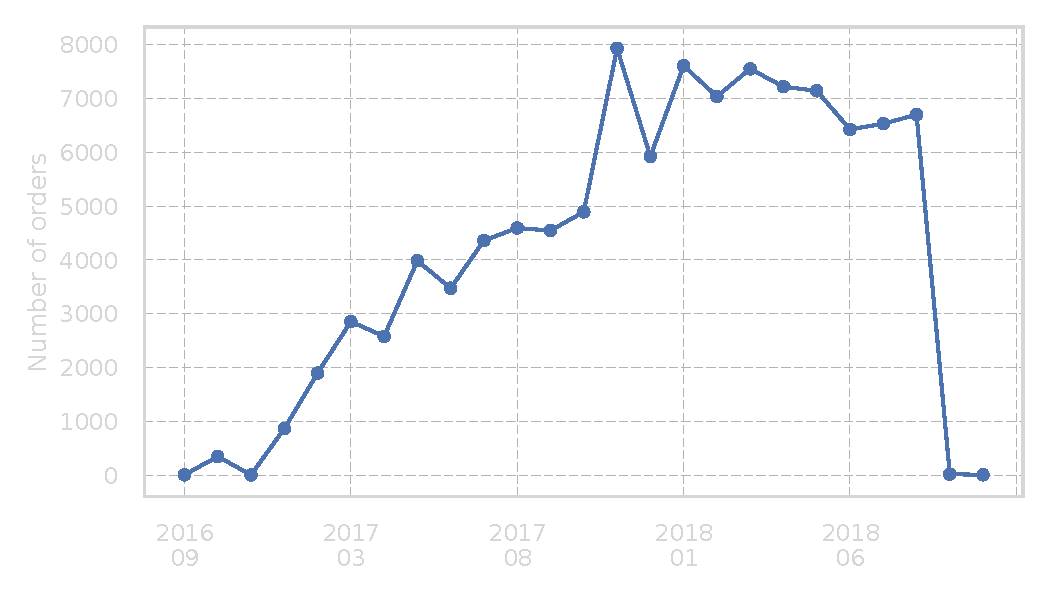
\includegraphics[width=90mm]{explore/N_orders_vs_time.pdf}} ;

		\visible<3>{
			\begin{scope}[xshift=87.7mm, yshift=31.5mm]
				\draw[myOrng, thick, rounded corners] ( 0,0 ) rectangle (8mm,4mm) ;
				\node[myOrng, text width=15mm, text centered] at (5mm, -4mm) {Questionner olist} ;
			\end{scope}
		}

		\visible<2->{
			\begin{scope}[yshift=1.5mm]
				\draw[myOrng, myarrow] (34mm, 32mm) -- (70mm, 60mm) ;
				\node[myOrng, text centered] at (70mm, 46mm) {Croissance importante} ;
			\end{scope}
		}
	\end{tikzpicture}
\end{frame}



\subsection{Statuts des commandes}

\begin{frame}[t, label=ordersStatus]
	\vspace{0mm}
	\begin{tikzpicture}
		\linespread{1}% <--- locally defined vertical line spacing in nodes
		\draw[clrBorders] (0,0) rectangle (\txw,\txh) ;
		\nodePageNumber

		\node[myShaded] at (\midX,83mm) {Statuts des commandes} ;
		\node at (\midX,\midY) {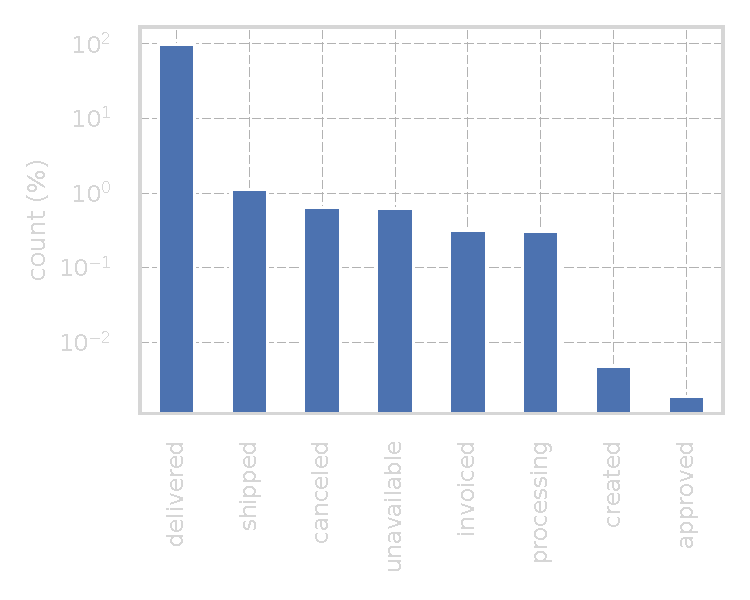
\includegraphics[width=90mm]{explore/order_status.pdf}} ;

		\visible<2>{
			\draw[myOrng, rounded corners, thick] (26.5mm, 15mm) rectangle (34mm,78mm) ;
			\node[myOrng, text width=30mm] at (51mm, 71mm) {Les commandes sont majoritairement livrées} ;
		}
	\end{tikzpicture}
\end{frame}



\subsection{Variables RFM}

\begin{frame}[t, label=varsRFM]
	\vspace{0mm}
	\begin{tikzpicture}
		\linespread{1}% <--- locally defined vertical line spacing in nodes
		\draw[clrBorders] (0,0) rectangle (\txw,\txh) ;
		\nodePageNumber

		\onlystyle<2->{shadedTwo}{myShaded}
		\node[shadedTwo] at (\midX, 80mm) {Variables RFM : définition} ;

			
		\visible<2->{
			\node[box_style00] (P) at (\midX,70mm) {Dans une \alert{période donnée}} ;
		}

		\begin{scope}[yshift=-15mm]
			\visible<3->{
				\node[box_style00, text width=15mm, text=myOrng] (A) at (\midX-35mm,60mm) {Récence} ;
				\draw[myarrow] (P.south) -- ++(0,-7.5mm) -| (A) ;
				\node[text centered, text width=30mm] (A2) at (\midX-35mm,40mm) {Nombre de jours depuis la dernière commande } ;
				\draw[myarrow] (A) -- (A2) ;
			}
				
			\visible<4->{
				\node[box_style00, text width=15mm, text=myOrng] (B) at (\midX,60mm) {Fréquence} ;
				\draw[myarrow] (P) -- (B) ;
				\node[text centered, text width=30mm] (B2) at (\midX,40mm) {Nombre de commandes} ;
				\draw[myarrow] (B) -- (B2) ;
			}
			\visible<5>{
				\node[box_style00, text width=15mm, text=myOrng] (C) at (\midX+35mm,60mm) {Montant} ;
				\draw[myarrow] (P.south) -- ++(0,-7.5mm) -| (C) ;
				\node[text centered, text width=30mm] (C2) at (\midX+35mm,40mm) { Somme des montants des commandes} ;
				\draw[myarrow] (C) -- (C2) ;
			}
		\end{scope}

	\end{tikzpicture}
\end{frame}

\begin{frame}[t, label=varRecence]
	\vspace{0mm}
	\begin{tikzpicture}
		\linespread{1}% <--- locally defined vertical line spacing in nodes
		\draw[clrBorders] (0,0) rectangle (\txw,\txh) ;
		\nodePageNumber

		\node[myShaded] at (\midX, 80mm) {Histogramme de la récence} ;
		\node at (\midX,\midY) {
\includegraphics[width=80mm] {explore/Recence.pdf}} ;

		\visible<2>{
		\node[myOrng, text width=40mm, text centered] at (\midX,13mm) {Proche de la courbe\\N~orders vs time (temps inversé)} ;
		}
	\end{tikzpicture}
\end{frame}


\begin{frame}[t, label=varFrequence]
	\vspace{0mm}
	\begin{tikzpicture}
		\linespread{1}% <--- locally defined vertical line spacing in nodes
		\draw[clrBorders] (0,0) rectangle (\txw,\txh) ;
		\nodePageNumber

		\node[myShaded] at (\midX, 80mm) {Histogramme de la fréquence} ;

		\node at (\midX,\midY) {
\includegraphics[width=80mm] {explore/Frequence.pdf}} ;

		\visible<2>{
			\node[myOrng, text width=70mm, text centered] at (\midX,15mm) {Principalement 1 commande par client (93.96\%)} ;
			% \draw[myarrow, myOrng] (40mm, 73mm) -- ++ (-11mm, -10mm) ;
			\draw[myOrng, thick, rounded corners] (26.5mm, 23mm) rectangle ( 29.3mm, 70mm ) ;
		}
	\end{tikzpicture}
\end{frame}


\begin{frame}[t, label=varMontant]
	\vspace{0mm}
	\begin{tikzpicture}
		\linespread{1}% <--- locally defined vertical line spacing in nodes
		\draw[clrBorders] (0,0) rectangle (\txw,\txh) ;
		\nodePageNumber

		\node[myShaded] at (\midX, 80mm) {Histogramme des montants} ;

		\node at (\midX,\midY) {
\includegraphics[width=80mm] {explore/Montant.pdf}} ;

		\visible<2>{
			\node[myOrng, text width=40mm, text centered] at (30mm,17.5mm) {Grande majorité de petits montants} ;
			\draw[myOrng, thick, rounded corners] (27mm, 24mm) rectangle ++ (6mm, 45.5mm) ;
		}
	\end{tikzpicture}
\end{frame}


\begin{frame}[t, label=pairplotRFM]
	\vspace{0mm}
	\begin{tikzpicture}
		\linespread{1}% <--- locally defined vertical line spacing in nodes
		\draw[clrBorders] (0,0) rectangle (\txw,\txh) ;
		\nodePageNumber

		\node[myShaded] at (\midX+20mm, 83mm) {Analyse bi-variée des variables RFM} ;

		\node at (\midX,\midY) {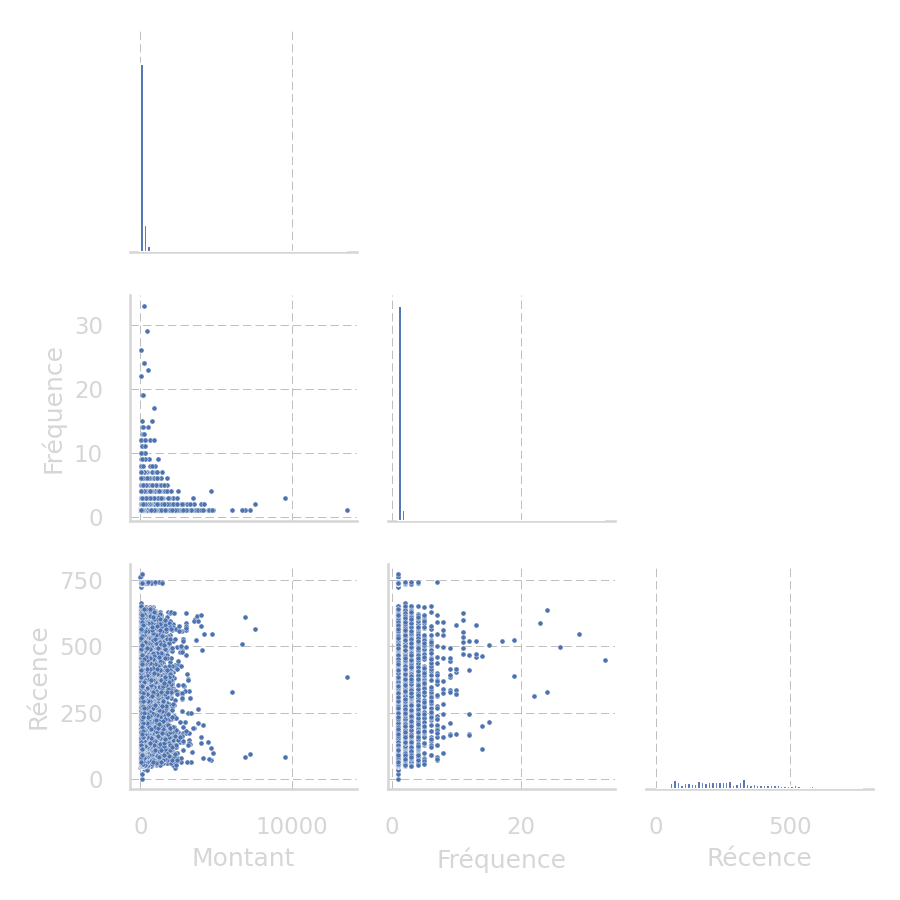
\includegraphics[width=80mm] {explore/pair_plot.png}} ;

		\visible<2->{
			\node[myOrng, text centered, text width=40mm] at (68mm,75mm) {Le montant est partiellement lié à la fréquence (inverse)} ;
			% \draw[myarrow, thick, myOrng] (28mm, 58mm) to [out=-90, in=180] (44mm, 42mm) ;
			\draw[myarrow, thick, myOrng] (28mm, 58mm) .. controls (29mm,43mm) .. (44mm, 42mm) ;
		}

		\visible<3>{
			\node[myOrng, text centered, text width=40mm] at (85mm,50mm) {Pas de lien direct\\récence - montant\\ou\\récence - fréquence} ;
			\draw[myOrng, thick, rounded corners] (25mm,15mm) rectangle ++ (22mm,22mm) ;
			\draw[myOrng, thick, rounded corners] (48mm,15mm) rectangle ++ (22mm,22mm) ;
		}

	\end{tikzpicture}
\end{frame}


\begin{frame}[t, label=RFMquantiles]
	\vspace{0mm}
	\begin{tikzpicture}
		\linespread{1}% <--- locally defined vertical line spacing in nodes
		\draw[clrBorders] (0,0) rectangle (\txw,\txh) ;
		\nodePageNumber

		\node at (\midX,80mm) {Séparation de chaque variable en 3 quantiles} ;
		\visible<2->{
			\node at (\midX+5mm,\midY) {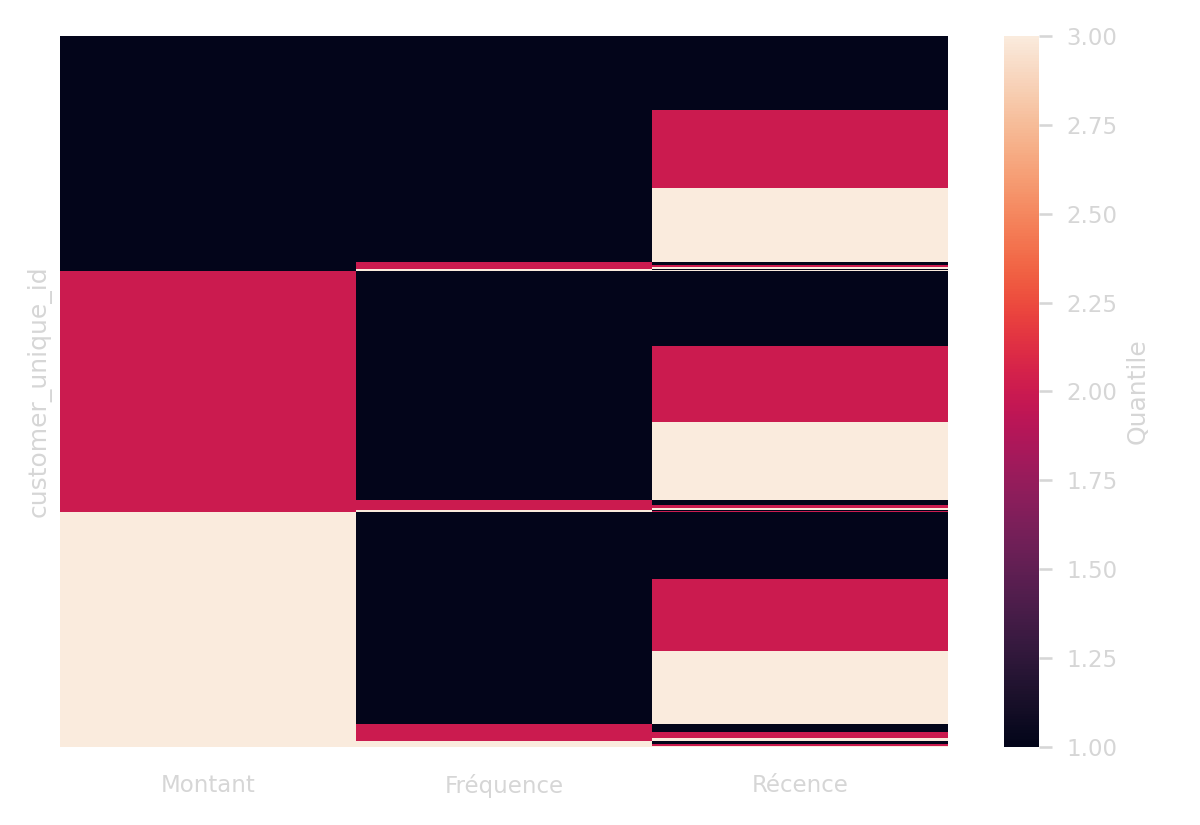
\includegraphics[width=70mm] {explore/quantiles.png}} ;
		}


		\visible<3>{
			\draw[myOrng, thick, rounded corners] (39mm+5.4mm, 22mm) rectangle ++(18mm, 47mm) ;
			\node[myOrng] at (\midX,15mm) {Faible proportion de fréquences élevées} ;
		}
	\end{tikzpicture}
\end{frame}


\subsection{Type de paiement}

\begin{frame}[t, label=varPaymentType]
	\vspace{0mm}
	\begin{tikzpicture}
		\linespread{1}% <--- locally defined vertical line spacing in nodes
		\draw[clrBorders] (0,0) rectangle (\txw,\txh) ;
		\nodePageNumber

		\node[myShaded] at (\midX, 80mm) {Type de paiement} ;

		\node at (\midX,\midY) {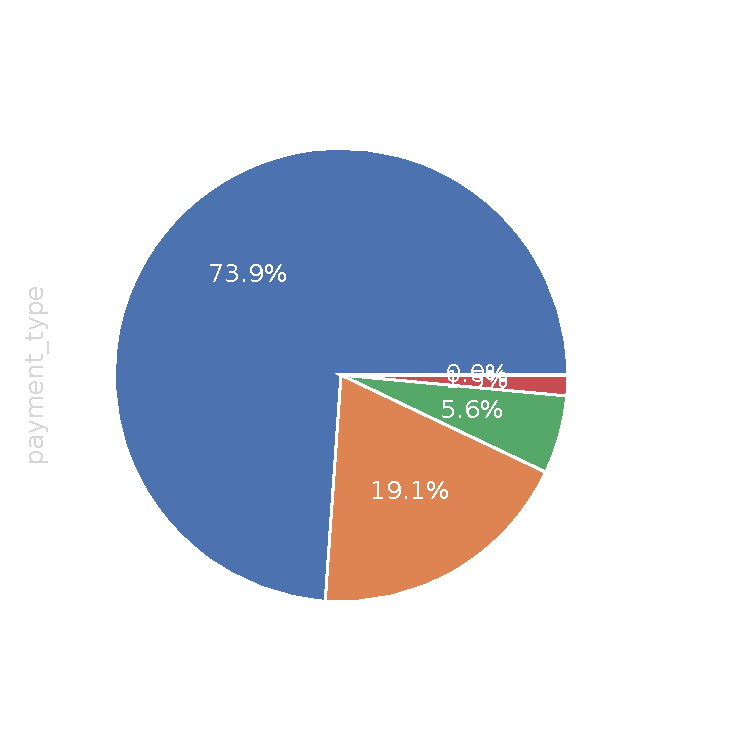
\includegraphics[width=80mm] {explore/payment_type.pdf}} ;

		\visible<2>{
			\node[myOrng, font=\bfseries] at (75mm, 75mm) {Majorité de "carte de crédit"} ;
		}
	\end{tikzpicture}
\end{frame}


\subsection{Avis sur les commandes}

\begin{frame}[t, label=varReviewScore]
	\vspace{0mm}
	\begin{tikzpicture}
		\linespread{1}% <--- locally defined vertical line spacing in nodes
		\draw[clrBorders] (0,0) rectangle (\txw,\txh) ;
		\nodePageNumber

		\node[myShaded] at (\midX,80mm) {Histogramme du review score} ;
		\node at (\midX,\midY) {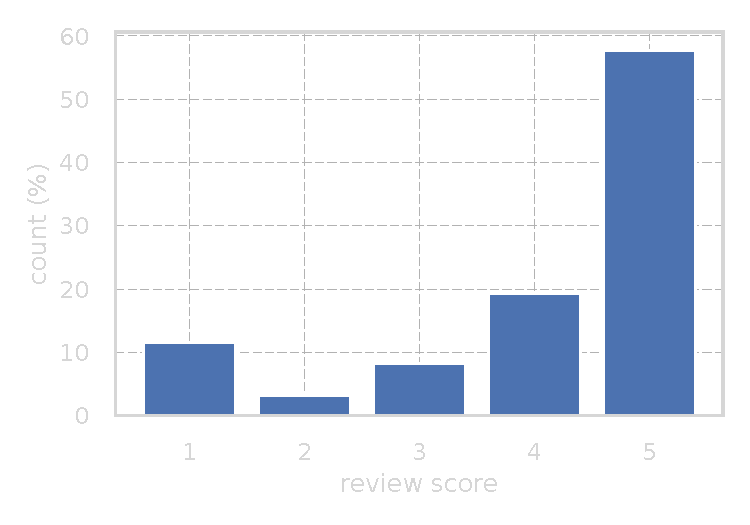
\includegraphics[width=80mm] {explore/review_score.pdf}} ;

		\visible<2>{
			\node[myOrng] at (80mm,18mm) {plus de 75\% $\geqslant$ 4 } ;
			\draw[myOrng, thick, rounded corners] (65mm, 29mm) rectangle ( 89.5mm, 70mm) ;
		}
	\end{tikzpicture}
\end{frame}


\subsection{Retards de livraison}

\begin{frame}[t, label=varDeliveryDelay]
	\vspace{0mm}
	\begin{tikzpicture}
		\linespread{1}% <--- locally defined vertical line spacing in nodes
		\draw[clrBorders] (0,0) rectangle (\txw,\txh) ;
		\nodePageNumber

		\visible<1-2>{
			\node[myShaded] at (\midX,80mm) {Histogramme du retard de livraison} ;
			\node at (\midX,\midY) {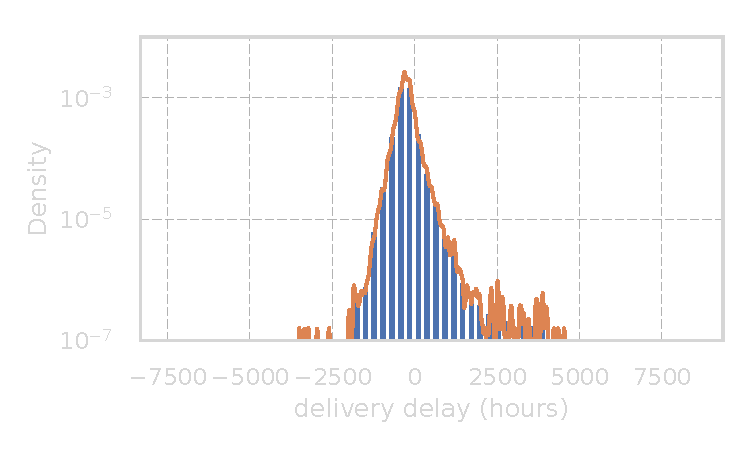
\includegraphics[width=80mm] {explore/delivery_delay.pdf}} ;
		}
		\visible<2>{
			\node[myOrng] at (\midX,15mm) {Distribution centrée autour de 0} ;
		}
		\visible<3->{
			\node[myShaded] at (\midX,80mm) {Fréquence \tit{vs} retard de livraison} ;
			\node at (\midX,\midY) {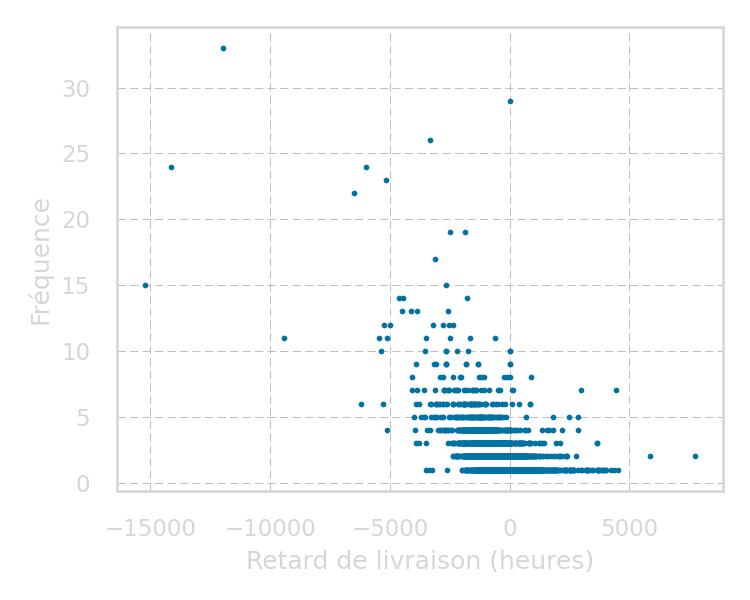
\includegraphics[width=80mm] {explore/delivery_delay_vs_frequency.png}} ;
		}
		\visible<4>{
			\node[myOrng] at (75mm,50mm) {Corrélation partielle} ;
			\draw[myarrow, myOrng, thick] (65mm, 45mm) .. controls (70mm, 33mm) .. (83mm,28mm) ;
		}

	\end{tikzpicture}
\end{frame}


\section{ESSAIS AVEC DIFFÉRENTS MODÈLES - VARIABLES RFM}

\subsection{ DBSCAN }

\begin{frame}[t, label=DBSCAN]
	\vspace{0mm}
	\begin{tikzpicture}
		\linespread{1}% <--- locally defined vertical line spacing in nodes
		\draw[clrBorders] (0,0) rectangle (\txw,\txh) ;
		\nodePageNumber

		\visible<1-5>{
			\node at (90mm,75mm) {
\includegraphics[width=30mm] {essais/dbscan/pie.pdf}} ;
		}

		\visible<2-3>{
			\node at (\midX,\midY) {
\includegraphics[width=80mm] {essais/dbscan/LDA.png}} ;
		}
		\visible<3>{
			\node[box_style00, myOrng, text width=22mm] at (60mm,70mm) {Séparations\\peu visibles} ;
		}

		\visible<4-5>{
			\node at (\midX,\midY) {
\includegraphics[width=80mm] {essais/dbscan/pairplot.png}} ;
		}
		\visible<5>{
			\node[box_style00, myOrng, text width=33mm] at (60mm,70mm) {Séparation principale:\\fréquence - montant} ;
		}

		\visible<6-9>{
			\node[myShaded] at (\midX,85mm) {TSNE} ;
			\node at (\midX,\midY+5mm) {
\includegraphics[width=60mm] {essais/dbscan/tsne.png}} ;
		}
		\visible<7->{
			\node[box_style00, myOrng] at (70mm,80mm) {TSNE stable} ;
		}

		\visible<8->{
			\node[text width=70mm, text centered] at (\midX,15mm) {Séparation \alert{correcte} par rapport à la \alert{TSNE}} ;
		}
		\visible<9>{
			\node[text width=90mm, text centered] at (\midX,10mm) {\alert{non actionnable} car \alert{peu exploitable} pour les \alert{variables initiales}} ;
		}
	\end{tikzpicture}
\end{frame}



\subsection{ Agglomerative clustering }

\begin{frame}[t, label=AgglomerativeClustering]
	\vspace{0mm}
	\begin{tikzpicture}
		\linespread{1}% <--- locally defined vertical line spacing in nodes
		\draw[clrBorders] (0,0) rectangle (\txw,\txh) ;
		\nodePageNumber

		\visible<1-5>{
			\node at (90mm,75mm) {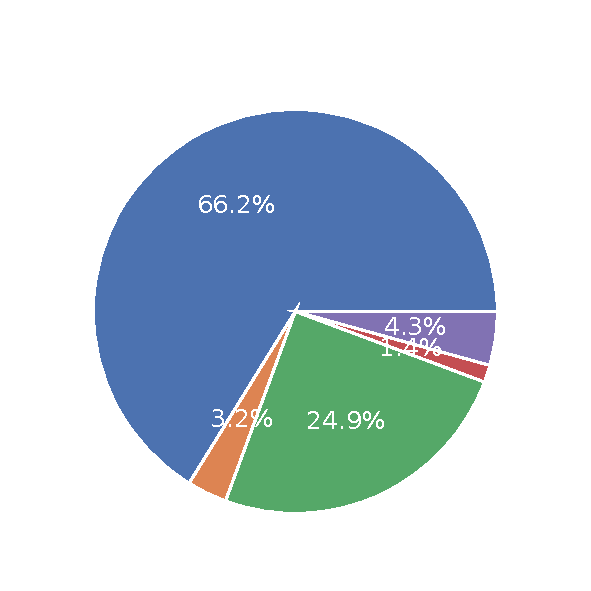
\includegraphics[width=30mm] {essais/agglomerative/pie.pdf}} ;
		}

		\visible<2-3>{
			\node at (\midX,\midY) {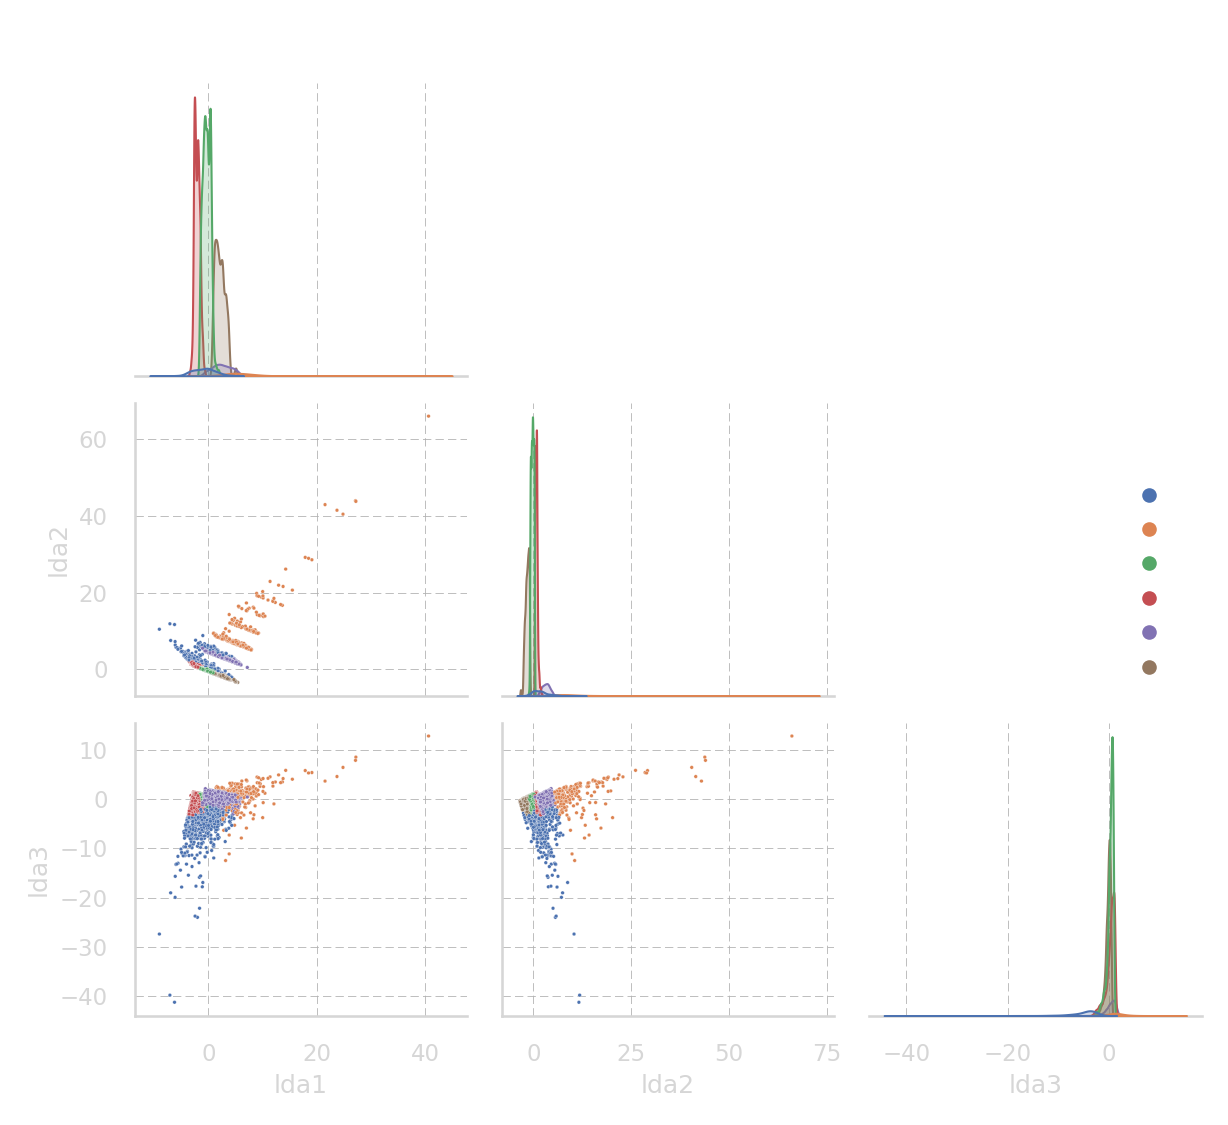
\includegraphics[width=80mm] {essais/agglomerative/LDA.png}} ;
		}
		\visible<3>{
			\node[box_style00, myOrng, text width=20mm] at (60mm,70mm) {Séparations partiellement visibles} ;
		}

		\visible<4-5>{
			\node at (\midX,\midY) {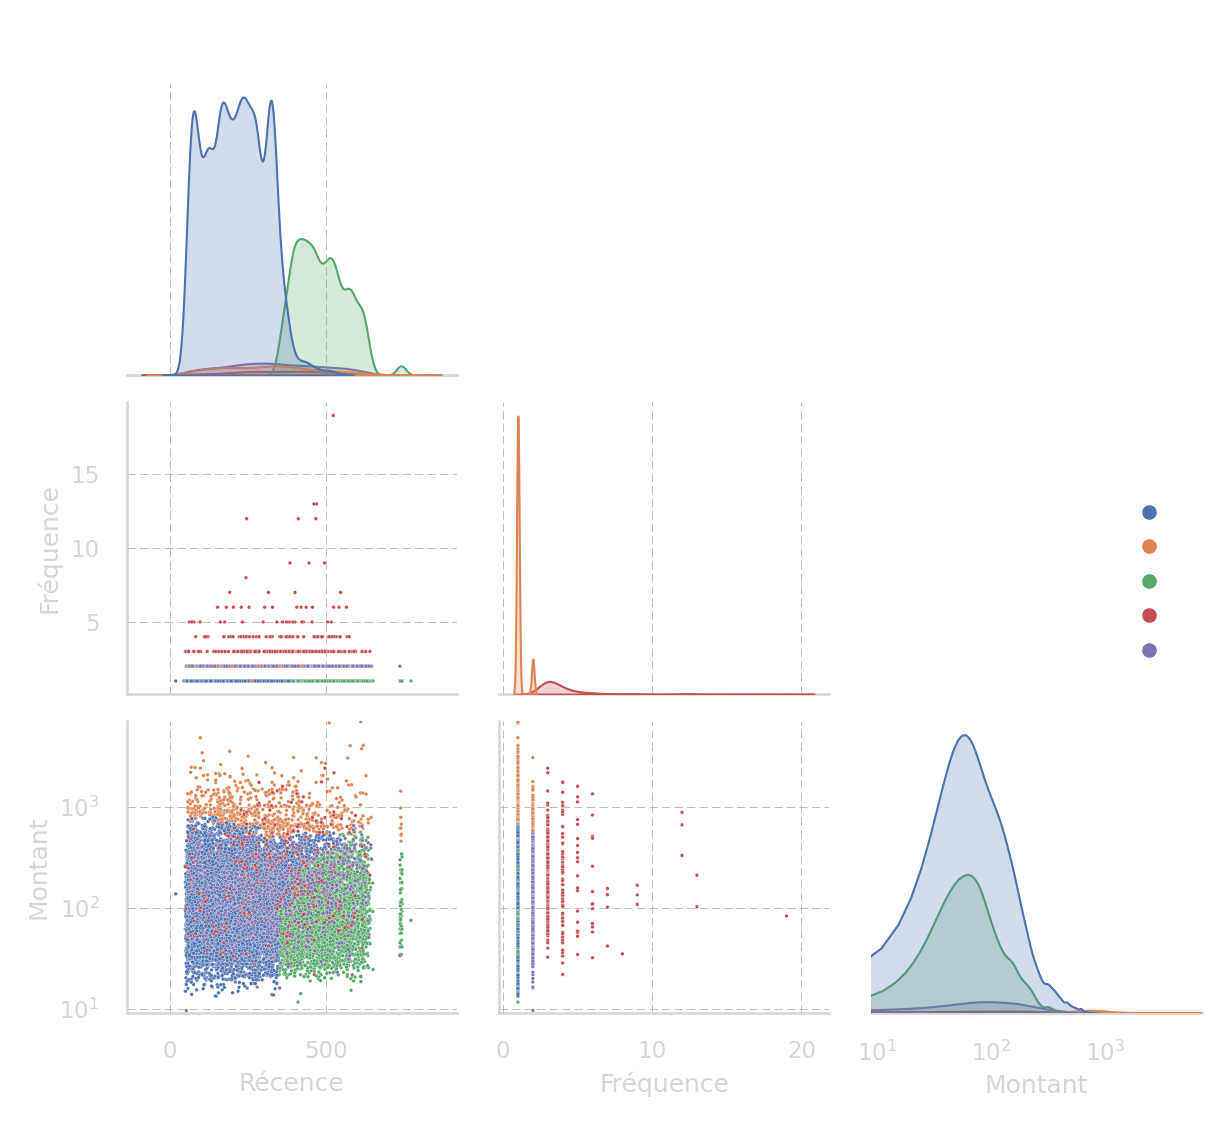
\includegraphics[width=80mm] {essais/agglomerative/pairplot.png}} ;
		}
		\visible<5>{
			\node[box_style00,myOrng, text width=33mm] at (60mm,70mm) {Séparations visuellement mieux exploitables} ;
			\draw[myOrng, rounded corners, thick] (25mm, 18mm) rectangle ++(16mm,10mm) ;
			\draw[myOrng, rounded corners, thick] (25mm, 28.5mm) rectangle ++(16mm,5mm) ;
			\draw[myOrng, rounded corners, thick] (47mm, 18mm) rectangle ++(16mm,15mm) ;
		}

		\visible<6-9>{
			\node[myShaded] at (\midX,85mm) {TSNE} ;
			\node at (\midX,\midY+5mm) {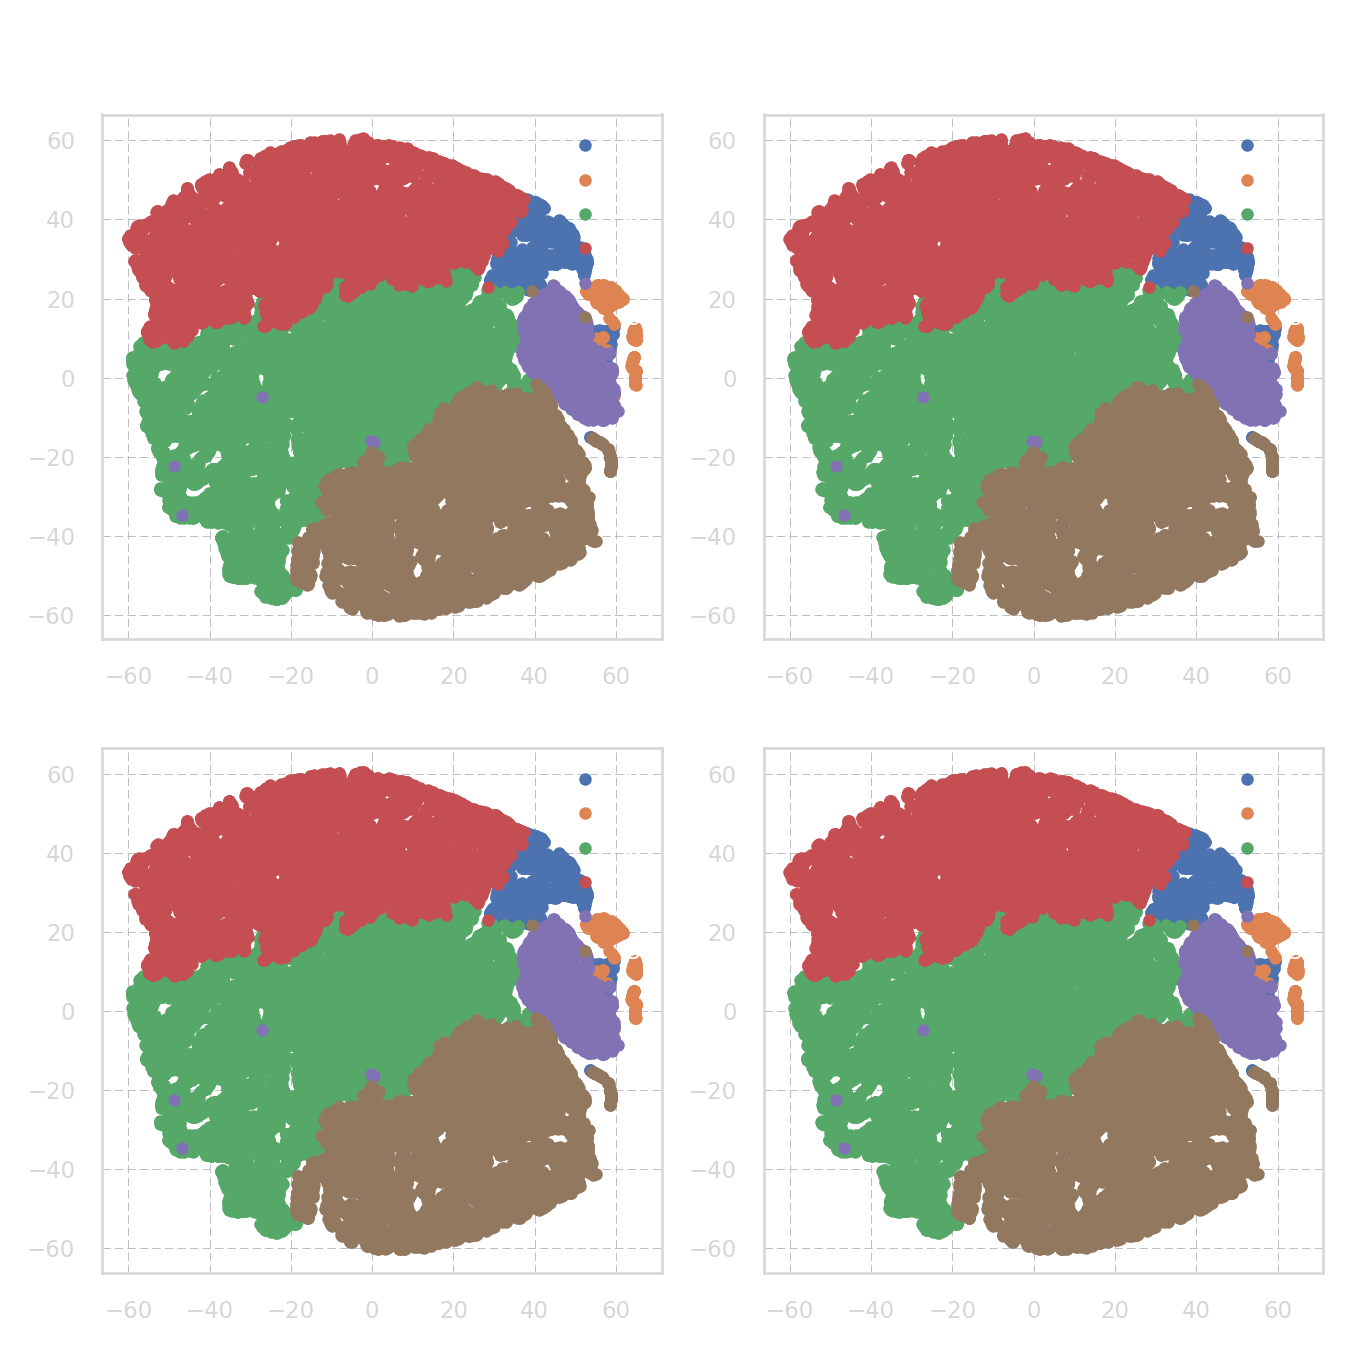
\includegraphics[width=60mm] {essais/agglomerative/tsne.png}} ;
		}
		\visible<7->{
			\node[box_style00, myOrng, text width=35mm] at (85mm,82mm) {Segmentation cohérente\\avec la TSNE} ;
		}

		\visible<8->{
			\node[text width=70mm, text centered] at (\midX,15mm) {Séparation \alert{cohérente} et \alert{compréhensible}} ;
		}
		\visible<9>{
			\node[text width=90mm, text centered] at (\midX,10mm) {\alert{mieux actionnable} que pour DBSCAN} ;
		}
	\end{tikzpicture}
\end{frame}



\subsection{ K-means }

\begin{frame}[t, label=KmeansSilhouette]
	\vspace{0mm}
	\begin{tikzpicture}
		\linespread{1}% <--- locally defined vertical line spacing in nodes
		\draw[clrBorders] (0,0) rectangle (\txw,\txh) ;
		\nodePageNumber

		\node[myShaded] at (\midX,80mm) {Visiualisation du score silhouette} ;

		\visible<2>{
			\node at (\midX,\midY) {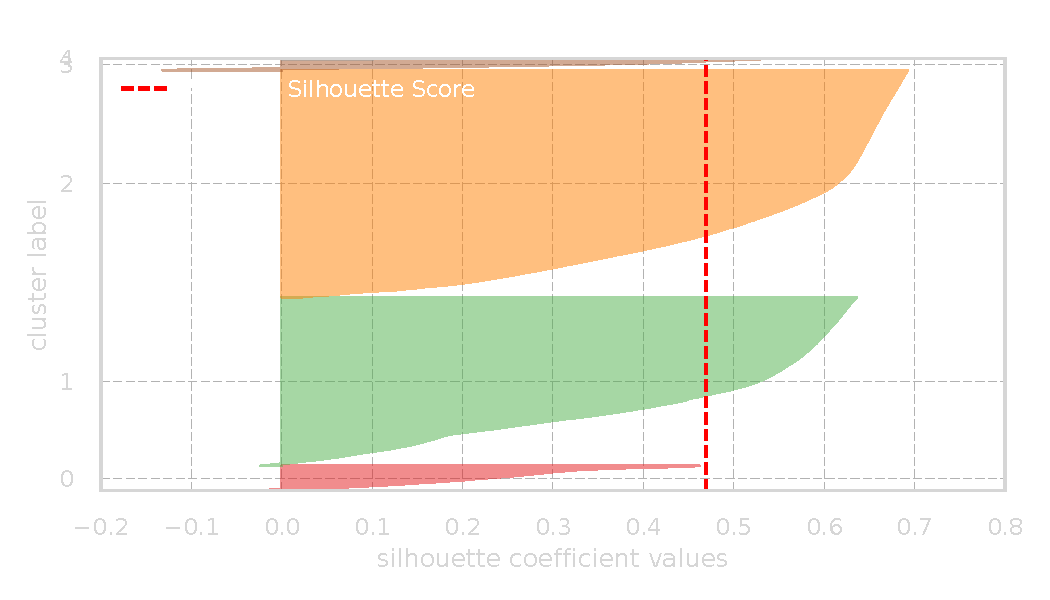
\includegraphics[width=80mm]{essais/silhouette_KM_optim.pdf}} ;
		}
		\visible<3->{
			\node at (\midX,\midY) {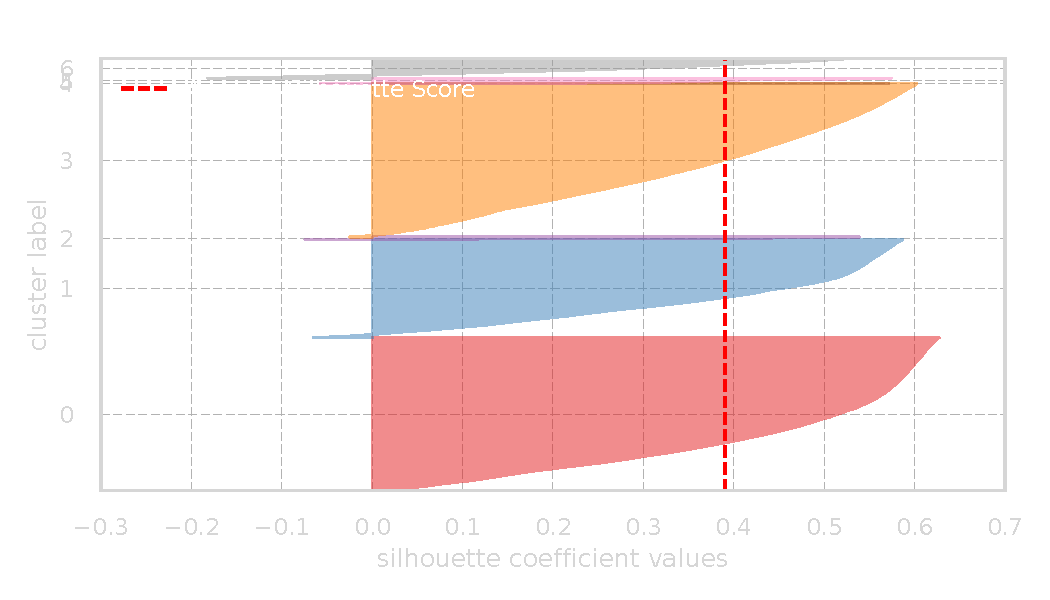
\includegraphics[width=80mm]{essais/silhouette_KM_sup.pdf}} ;
		}
		\visible<1>{
			\node at (\midX,\midY) {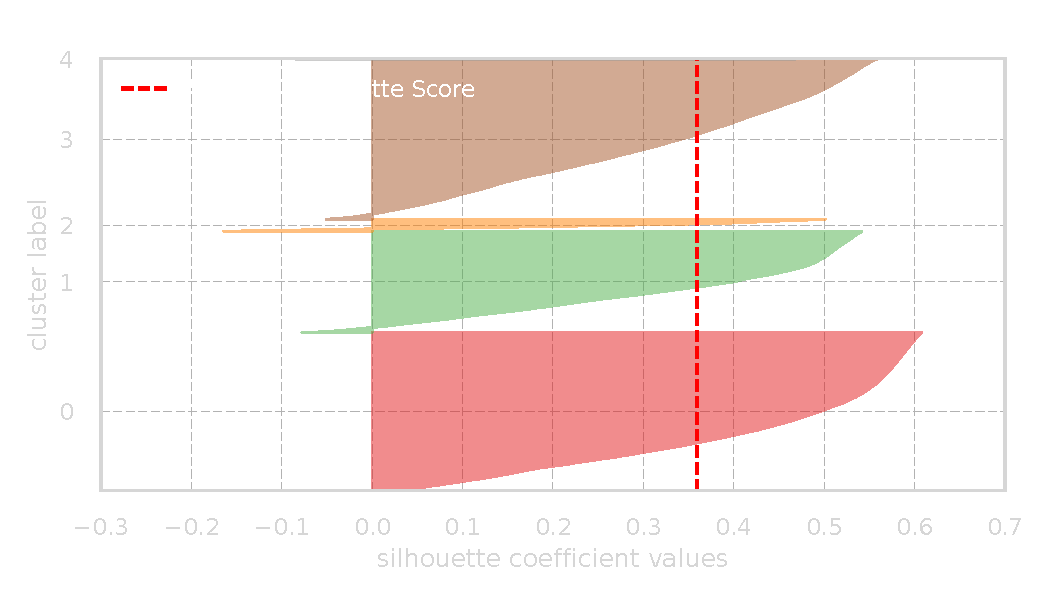
\includegraphics[width=80mm]{essais/silhouette_KM_sub.pdf}} ;
		}

		\visible<4>{
			\node[myOrng] at (\midX,15mm) {Résultats globalement cohérents} ;
		}

	\end{tikzpicture}
\end{frame}

\begin{frame}[t, label=Kmeans]
	\vspace{0mm}
	\begin{tikzpicture}
		\linespread{1}% <--- locally defined vertical line spacing in nodes
		\draw[clrBorders] (0,0) rectangle (\txw,\txh) ;
		\nodePageNumber

		\visible<1-5>{
			\node at (90mm,75mm) {
\includegraphics[width=30mm] {essais/k_elbow_optim/pie.pdf}} ;
		}
			
		\visible<1>{
			\node[myShaded] at (40mm,85mm) {Diagramme polaire du centre des clusters} ;
			\node at (40mm, \midY) { 
\includegraphics[width=70mm] {essais/k_elbow_optim/polar_centers.pdf} } ;
		}

		\visible<2-3>{
			\node at (\midX,\midY) {
\includegraphics[width=80mm] {essais/k_elbow_optim/LDA.png}} ;
		}
		\visible<3>{
			\node[box_style00, myOrng, text width=20mm] at (60mm,70mm) {Séparations bien visibles} ;
		}

		\visible<4-5>{
			\node at (\midX,\midY) {
\includegraphics[width=80mm] {essais/k_elbow_optim/pairplot.png}} ;
		}
		\visible<5>{
			\node[box_style00, myOrng, text width=33mm] at (60mm,70mm) {Séparations visuellement\\bien exploitables} ;
			\draw[myOrng, rounded corners, thick] (25mm, 18mm) rectangle ++(16mm,10mm) ;
			\draw[myOrng, rounded corners, thick] (25mm, 28.5mm) rectangle ++(16mm,5mm) ;
			\draw[myOrng, rounded corners, thick] (47mm, 18mm) rectangle ++(16mm,15mm) ;
		}

		\visible<6-9>{
			\node[myShaded] at (\midX,85mm) {TSNE} ;
			\node at (\midX,\midY+5mm) {
\includegraphics[width=60mm] {essais/k_elbow_optim/tsne.png}} ;
		}
		\visible<7->{
			\node[box_style00, myOrng, text width=40mm] at (85mm,83mm) {Segmentation partiellement cohérente avec la TSNE} ;
		}

		\visible<8->{
			\node[text width=70mm, text centered] at (\midX,15mm) {Séparation \alert{cohérente} et \alert{compréhensible}} ;
		}
		\visible<9>{
			\node[text width=90mm, text centered] at (\midX,10mm) {\alert{mieux actionnable} que pour DBSCAN et le clustering agglomératif} ;
		}
	\end{tikzpicture}
\end{frame}




\section{ ESSAIS D'AJOUTS DE VARIABLES }

\subsection{ Retards de livraison }

\begin{frame}[t, label=KmeansDelay]
	\vspace{0mm}
	\begin{tikzpicture}
		\linespread{1}% <--- locally defined vertical line spacing in nodes
		\draw[clrBorders] (0,0) rectangle (\txw,\txh) ;
		\nodePageNumber

		\visible<1-5>{
			\node at (90mm,75mm) {
\includegraphics[width=30mm] {essais/delay/k_elbow_optim/pie.pdf}} ;
		}

		\visible<1>{
			\node[myShaded] at (40mm,85mm) {Diagramme polaire du centre des clusters} ;
			\node at (40mm, \midY) { 
\includegraphics[width=70mm] {essais/delay/k_elbow_optim/polar_centers.pdf} } ;
		}

		\visible<2-3>{
			\node at (\midX,\midY) {
\includegraphics[width=80mm] {essais/delay/k_elbow_optim/LDA.png}} ;
		}
		\visible<3>{
			\node[box_style00, myOrng, text width=20mm] at (60mm,70mm) {Séparations bien visibles} ;
		}

		\visible<4-5>{
			\node at (\midX,\midY) {
\includegraphics[width=80mm] {essais/delay/k_elbow_optim/pairplot.png}} ;
		}
		\visible<5>{
			\node[box_style00,myOrng, text width=33mm] at (58mm,70mm) {Séparations visuellement\\exploitables} ;
			% \draw[myOrng, rounded corners, thick] (25mm, 18mm) rectangle ++(16mm,10mm) ;
			% \draw[myOrng, rounded corners, thick] (25mm, 28.5mm) rectangle ++(16mm,5mm) ;
			\draw[myOrng, rounded corners, thick] (41mm, 15mm) rectangle ++(15mm,14.5mm) ;
			\draw[myOrng, myarrow](43mm,28mm) .. controls (45mm, 24.5mm) .. (50mm, 22mm) ;
		}

		\visible<6->{
			\node[myShaded] at (\midX,85mm) {TSNE} ;
			\node at (\midX,\midY+5mm) {
\includegraphics[width=60mm] {essais/delay/k_elbow_optim/tsne.png}} ;
		}
		\visible<7->{
			\node[box_style00, myOrng, text width=40mm] at (82mm,85mm) {Segmentation partiellement cohérente avec la TSNE} ;
		}

		\visible<8->{
			\node[text width=70mm, text centered] at (\midX,15mm) {Séparation \alert{cohérente} et \alert{compréhensible}} ;
		}
		\visible<9>{
			\node[text width=90mm, text centered] at (\midX,10mm) {\alert{actionnable}, mais \tit{quid} de la \alert{pertinence} pour la segmentation ?} ;
		}
	\end{tikzpicture}
\end{frame}

\subsection{ Avis sur la commande }

\begin{frame}[t, label=KmeansReviewScore]
	\vspace{0mm}
	\begin{tikzpicture}
		\linespread{1}% <--- locally defined vertical line spacing in nodes
		\draw[clrBorders] (0,0) rectangle (\txw,\txh) ;
		\nodePageNumber

		\visible<1-5>{
			\node at (90mm,75mm) {
\includegraphics[width=30mm] {essais/review_score/k_elbow_optim/pie.pdf}} ;
		}

		\visible<1>{
			\node[myShaded] at (40mm,85mm) {Diagramme polaire du centre des clusters} ;
			\node at (40mm, \midY) { 
\includegraphics[width=70mm] {essais/review_score/k_elbow_optim/polar_centers.pdf} } ;
		}

		\visible<2-3>{
			\node at (\midX,\midY) {
\includegraphics[width=80mm] {essais/review_score/k_elbow_optim/LDA.png}} ;
		}
		\visible<3>{
			\node[box_style00, myOrng, text width=20mm] at (60mm,70mm) {Séparations bien visibles} ;
		}

		\visible<4-5>{
			\node at (\midX,\midY) {
\includegraphics[width=80mm] {essais/review_score/k_elbow_optim/pairplot.png}} ;
		}
		\visible<5>{
			\node[box_style00, myOrng, text width=30mm] at (58mm,70mm) {Séparation des faibles\\review scores} ;
			\draw[myOrng, rounded corners, thick] (75.5mm, 13.5mm) rectangle ++(18mm,16mm) ;
			% \draw[myOrng, rounded corners, thick] (25mm, 28.5mm) rectangle ++(16mm,5mm) ;
			% \draw[myOrng, rounded corners, thick] (41mm, 15mm) rectangle ++(15mm,14.5mm) ;
			% \draw[myOrng, myarrow](43mm,28mm) .. controls (45mm, 24.5mm) .. (50mm, 22mm) ;
		}

		\visible<6->{
			\node[myShaded] at (\midX,85mm) {TSNE} ;
			\node at (\midX,\midY+5mm) {
\includegraphics[width=60mm] {essais/delay/k_elbow_optim/tsne.png}} ;
		}
		\visible<7->{
			\node[box_style00, myOrng, text width=40mm] at (82mm,84mm) {Présence d'incohérences avec la TSNE} ;
		}

		\visible<8->{
			\node[text width=70mm, text centered] at (\midX,15mm) {Séparation \alert{cohérente} et \alert{realativement compréhensible}} ;
		}
		\visible<9>{
			\node[text width=90mm, text centered] at (\midX,10mm) {\alert{actionnable}, mais \tit{quid} de la \alert{pertinence} pour la segmentation ?} ;
		}
	\end{tikzpicture}
\end{frame}



\subsection{ Type de paiement }

\begin{frame}[t, label=KmeansPaymentType]
	\vspace{0mm}
	\begin{tikzpicture}
		\linespread{1}% <--- locally defined vertical line spacing in nodes
		\draw[clrBorders] (0,0) rectangle (\txw,\txh) ;
		\nodePageNumber

		\visible<1-6>{
			\node at (90mm,75mm) {
\includegraphics[width=30mm] {essais/payment_type/k_elbow_optim/pie.pdf}} ;
		}

		\visible<1-2>{
			\node[myShaded] at (40mm,85mm) {Diagramme polaire du centre des clusters} ;
			\node at (40mm, \midY) { 
\includegraphics[width=70mm] {essais/payment_type/k_elbow_optim/polar_centers.pdf} } ;
			\visible<2>{
				\node[myOrng, text width=30mm, text centered] at (85mm,20mm) {Impact très important sur les clusters} ;
			}
		}

		\visible<3-4>{
			\node at (\midX,\midY) {
\includegraphics[width=80mm] {essais/payment_type/k_elbow_optim/LDA.png}} ;
		}
		\visible<4>{
			\node[box_style00, myOrng, text width=20mm] at (60mm,70mm) {Séparations non visibles sur 3 variables} ;
		}

		\visible<5-6>{
			\node at (\midX,\midY) {
\includegraphics[width=80mm] {essais/payment_type/k_elbow_optim/pairplot.png}} ;
		}
		\visible<6>{
			\node[box_style00, myOrng, text width=25mm] at (60mm,70mm) {Séparations\\relativement\\peu lisibles} ;
			% \draw[myOrng, rounded corners, thick] (25mm, 18mm) rectangle ++(16mm,10mm) ;
			% \draw[myOrng, rounded corners, thick] (25mm, 28.5mm) rectangle ++(16mm,5mm) ;
			% \draw[myOrng, rounded corners, thick] (41mm, 15mm) rectangle ++(15mm,14.5mm) ;
			% \draw[myOrng, myarrow](43mm,28mm) .. controls (45mm, 24.5mm) .. (50mm, 22mm) ;
		}

		\visible<7->{
			\node[myShaded] at (\midX,85mm) {TSNE} ;
			\node at (\midX,\midY+5mm) {
\includegraphics[width=60mm] {essais/delay/k_elbow_optim/tsne.png}} ;
		}
		\visible<8->{
			\node[box_style00, myOrng, text width=40mm] at (82mm,84mm) {Présence d'incohérences avec la TSNE} ;
		}

		\visible<9->{
			\node[text width=70mm, text centered] at (\midX,15mm) {Séparation \alert{fortement liée} au \alert{type} de paiement} ;
		}
		\visible<10>{
			\node[text width=90mm, text centered] at (\midX,10mm) {\alert{Pas nécessairement actionnable}} ;
		}
	\end{tikzpicture}
\end{frame}


\subsection{Conclusions}

\begin{frame}[t, label=EssaisCCL]
	\vspace{0mm}
	\begin{tikzpicture}
		\linespread{1}% <--- locally defined vertical line spacing in nodes
		\draw[clrBorders] (0,0) rectangle (\txw,\txh) ;
		\nodePageNumber

		\node[box_style00, text width=40mm] at (0.25\txw,70mm) {L'algorithme \alert{K-means} est plus \alert{pertinent} que le DBSCAN et l'agglomerative clustering} ;

		\visible<2->{
			\node[box_style00, text width=40mm] at (0.75\txw,70mm) {Les variables \alert{RFM} permettent une \alert{segmentation actionnable} } ;
		}
		
		\visible<3->{
			\node[box_style00, text width=40mm] (A) at (0.25\txw,40mm) { Les variables "delivery delay", "review score" et "payment type" apportent des \alert{informations intéressantes} } ;
		}
		\visible<4->{
			\node[box_style00, text width=40mm] (B) at (0.25\txw,20mm) {\alert{Pertinence moindre} pour la \alert{segmentation} } ;
		}

		\visible<5->{
			\node[box_style00, text width=40mm] (C) at (0.75\txw,30mm) {\alert{À discuter} avec l'équipe marketing d'Olist} ;
			\draw[myarrow] (A) -| (C) ;
			\draw[myarrow] (B) -| (C) ;
		}


	\end{tikzpicture}
\end{frame}


\section{CONTRAT DE MAINTENANCE}

\subsection{Protocole}
\begin{frame}[t, label=MaintenanceProtocole]
	\vspace{0mm}
	\begin{tikzpicture}
		\linespread{1}% <--- locally defined vertical line spacing in nodes
		\draw[clrBorders] (0,0) rectangle (\txw,\txh) ;
		\nodePageNumber

		\node[myShaded] at (\midX,85mm) {Protocole} ;
		\begin{scope}[ xshift=5mm, yshift=-10mm]

			\visible<2->{
				\node[box_style00, myOrng] (M0) at (80mm,80mm) {$M_0$ } ;
				\node[box_style00, left=of M0] (T0) { Entrainement } ;
			}

			\node[box_style00, text width=25mm, left=of T0] (D0) {Données\\ $[T_0$, $T_0$ + durée ]} ;

			\visible<2->{
				\draw[myarrow] (D0) -- (T0) ;
				\draw[myarrow] (T0) -- (M0) ;
			}

			\visible<4->{
				\node[box_style00, below=of M0] (P0) {Prédiction} ;
				\node[box_style00, below=of P0, myOrng] (L0) {$L_0$} ;
			}

			\visible<3->{
				\node[box_style00, text width=25mm, left=of P0] (Di) {Données\\ $[T_i$, $T_i$ + durée ]} ;
			}

			\visible<4->{
				\draw[myarrow] (M0) -- (P0) ;
				\draw[myarrow] (P0) -- (L0) ;
				\draw[myarrow] (Di) -- (P0) ;
			}

			\visible<7->{
				\node[box_style00, below=of L0] (ARI) {Score ARI} ;
			}

			\visible<6->{
				\node[box_style00, left=of ARI, myOrng] (Li) {$L_i$} ;
				\node[box_style00, left=of Li] (Pi) {Prédiction} ;
			}

			\visible<5->{
				\node[box_style00, left=of Pi, myOrng] (Mi) {$M_i$} ;
				\node[box_style00, above=of Mi] (Ti) { Entrainement } ;
				\draw[myarrow] (Di) -| (Ti) ;
				\draw[myarrow] (Ti) -- (Mi) ;
			}

			\visible<6->{
				\draw[myarrow] (Mi) -- (Pi) ;
				\draw[myarrow] (Pi) -- (Li) ;
				\draw[myarrow] (Di) -- ++ (0, -10mm) -| (Pi) ;
			}


			\visible<7->{
				\draw[myarrow] (L0) -- (ARI) ;
				\draw[myarrow] (Li) -- (ARI) ;
			}

			% \draw[myarrow] (Di) |- (P0) ;
			% \draw[myarrow, myOrng] (Di.east) -- ++(10mm,0) ;
		\end{scope}

		\visible<8>{
			\node[myOrng] at (\midX,15mm) {durée = 1 an} ;
			\node[myOrng] at (\midX,10mm) {$T_i$ = $T_0$ + i*(1 semaine)} ;
		}

	\end{tikzpicture}
\end{frame}


\subsection{Analyse des clusters initiaux}
\begin{frame}[t, label=MaintenancePairplots]
	\vspace{0mm}
	\begin{tikzpicture}
		\linespread{1}% <--- locally defined vertical line spacing in nodes
		\draw[clrBorders] (0,0) rectangle (\txw,\txh) ;
		\nodePageNumber

		\visible<1>{
			\node[myShaded] at (\midX,86mm) {Diagramme polaire des centres des clusters} ;
		\node at (\midX,\midY) {
\includegraphics[width=75mm] {simulations/k_means_initial_(k=4)/polar_centers.pdf}} ;
		}
		\visible<2-3>{
		\node at (\midX,\midY) {
\includegraphics[width=80mm] {simulations/k_4/pairplot.png}} ;
		\node at (80mm,70mm) {
\includegraphics[width=30mm] {simulations/k_4/pie.pdf}} ;
		}
		\visible<3>{
			\node[box_style00, myOrng, text width=25mm] at (55mm,70mm) {Segmentation\\cohérente avec les données précédentes} ;
		}

		\visible<4-5>{
			\node[myShaded] at (\midX,80mm) {Diagrammes polaires des centres des clusters} ;
		\node at (\midX-25mm,\midY) {
\includegraphics[width=50mm] {simulations/k_means_initial_(k=4)/polar_centers.pdf}} ;
		\node at (\midX+25mm,\midY) {
\includegraphics[width=50mm] {simulations/k_means_initial_(k=5)/polar_centers.pdf}} ;
		}
		\visible<5-7>{
			\node[myOrng] at (\midX,8mm) {Nouvelle séparation sur la fréquence} ;
		}
		\visible<6-7>{
		\node at (\midX,\midY) {
\includegraphics[width=80mm] {simulations/k_5/pairplot.png}} ;
		\node at (80mm,70mm) {
\includegraphics[width=30mm] {simulations/k_5/pie.pdf}} ;
		}
		\visible<7>{
			% \draw[myOrng, rounded corners, thick] (27mm, 30mm) rectangle (38.5mm, 36mm) ;
			% \draw[myOrng, rounded corners, thick] (47mm, 30mm) rectangle (49.5mm, 36mm) ;
			\draw[myOrng, rounded corners, thick] (26mm, 39mm) rectangle (40mm, 56mm) ;
			\draw[myOrng, rounded corners, thick] (48mm, 15mm) rectangle (65mm, 36mm) ;
		}

	\end{tikzpicture}
\end{frame}

\subsection{Courbe Adjusted Rand Index}
\begin{frame}[t, label=MaintenanceCurve]
	\vspace{0mm}
	\begin{tikzpicture}
		\linespread{1}% <--- locally defined vertical line spacing in nodes
		\draw[clrBorders] (0,0) rectangle (\txw,\txh) ;
		\nodePageNumber

		\node at (\midX,83.5mm) {Évolution du score ARI pour k=4} ;
		\node at (\midX,\midY+20mm) {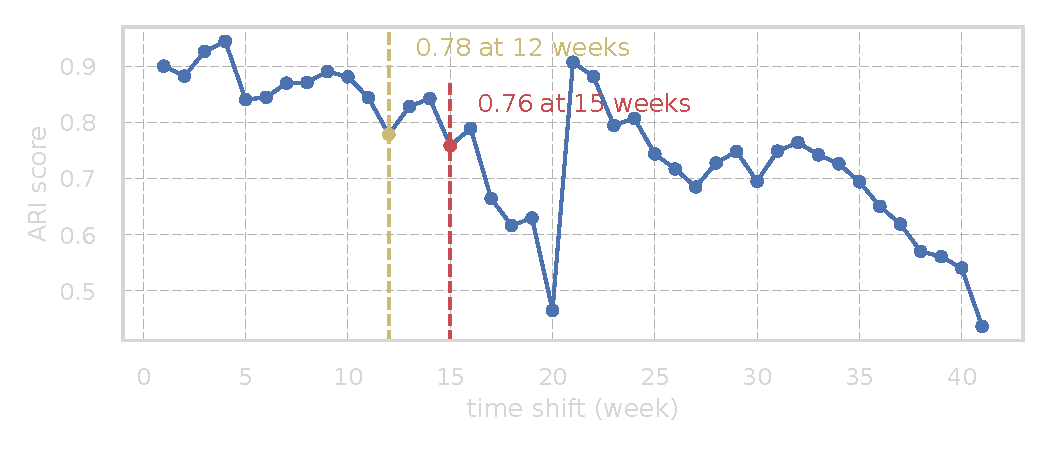
\includegraphics[width=80mm] {simulations/k_4/ARI.pdf}} ;

		\visible<2->{
			\node at (\midX,43.5mm) {Évolution du score ARI pour k=5} ;
			\node at (\midX,\midY-20mm) {
\includegraphics[width=80mm] {simulations/k_5/ARI.pdf}} ;
		}

		\visible<3>{
			\node[myOrng] at (\midX,7mm) {Les résultats sont \alert{similaires}} ;
		}
	\end{tikzpicture}
\end{frame}


\section{CONCLUSIONS}
\begin{frame}[t, label=CCL]
	\vspace{0mm}
	\begin{tikzpicture}
		\linespread{1}% <--- locally defined vertical line spacing in nodes
		\draw[clrBorders] (0,0) rectangle (\txw,\txh) ;
		\nodePageNumber

		\node[box_style00, text width=42mm, minimum height=10mm] (A)
			at (0.25*\txw, 70mm) {Algorithm \alert{K-means} sélectionné} ;
		\visible<2->{
			\node[box_style00, text width=42mm, minimum height=10mm] (B)
				at (0.75*\txw, 70mm) {Variables \alert{RFM}} ;
		}

		\visible<3->{
			\node[box_style00, text width=42mm, minimum height=10mm] (C)
				at (\midX,45mm) {Segmentation \alert{actionnable}\\clusters \alert{explicables}} ;
			\draw[myarrow] (A) -- ++ (0,-12mm) -| (C) ;
			\draw[myarrow] (B) -- ++ (0,-12mm) -| (C) ;
		}

		\visible<4>{
			\node[box_style00, text width=72mm, minimum height=10mm]
				at (\midX, 20mm) {\alert{Maintenance} :\\ $\bullet$ besoin à partir de \alert{15} ou \alert{24} semaines \rule{6.5mm}{0mm}\\ $\bullet$ besoins similaires pour \alert{4} ou \alert{5} clusters \rule{5.1mm}{0mm}} ;
		}

	\end{tikzpicture}
\end{frame}

\section{PERSPECTIVES}
\begin{frame}[t, label=Perspectives]
	\vspace{0mm}
	\begin{tikzpicture}
		\linespread{1}% <--- locally defined vertical line spacing in nodes
		\draw[clrBorders] (0,0) rectangle (\txw,\txh) ;
		\nodePageNumber

		\node[text centered] at (\midX,75mm) {Discussions avec Olist:} ;

		\visible<2->{
			\node[box_style00, text width=44mm, minimum height=15mm] at (0.26*\txw, 55mm) {Intérêts des \alert{variables ajoutables}} ;
		}
		\visible<3->{
			\node[box_style00, text width=44mm, minimum height=15mm] at (0.74*\txw, 55mm) {Besoins sur le \alert{nombre de groupes}} ;
		}
		\visible<4->{
			\node[box_style00, text width=44mm, minimum height=15mm] at (0.26*\txw, 30mm) {Possibilités en terme de \alert{maintenance}} ;
		}
		\visible<5>{
			\node[box_style00, text width=44mm, minimum height=15mm] at (0.74*\txw, 30mm) {\alert{Avis} experts métiers} ;
		}

	\end{tikzpicture}
\end{frame}


\begin{frame}[t, label=Merci]
	\vspace{0mm}
	\begin{tikzpicture}
		\linespread{1}% <--- locally defined vertical line spacing in nodes
		\draw[clrBorders] (0,0) rectangle (\textwidth,\textheight) ;

		\node at (0.5\textwidth,\midY) {\huge \alert{Merci} pour votre \alert{attention}.} ;

	\end{tikzpicture}
\end{frame}


\end{document}
